%% ****** Start of file aiptemplate.tex ****** %
%%
%%   This file is part of the files in the distribution of AIP substyles for REVTeX4.
%%   Version 4.1 of 9 October 2009.
%%
%
% This is a template for producing documents for use with 
% the REVTEX 4.1 document class and the AIP substyles.
% 
% Copy this file to another name and then work on that file.
% That way, you always have this original template file to use.

\documentclass[aip, pop, preprint]{revtex4-1}
%\documentclass[aip,preprint]{revtex4-1}


% Include some handy packages
\usepackage{amssymb,amsmath,color}
\usepackage{graphicx}
%\usepackage{wrapfig}
%\usepackage{caption}
%\usepackage{subcaption}
%\usepackage{placeins}
%\usepackage{setspace}
\usepackage{xfrac}
%\usepackage{pdfpages}

%\draft % marks overfull lines with a black rule on the right

\begin{document}
\graphicspath{{figures/}{plots/}}

% Use the \preprint command to place your local institutional report number 
% on the title page in preprint mode.
% Multiple \preprint commands are allowed.
%\preprint{}

%\title{Investigation into Classical Ion Heat Transport in Enhanced-Confinement MST Plasmas using Integrated Forward Modeling} %Title of paper
\title{Classical ion heat transport in RFP plasmas}
% repeat the \author .. \affiliation  etc. as needed
% \email, \thanks, \homepage, \altaffiliation all apply to the current author.
% Explanatory text should go in the []'s, 
% actual e-mail address or url should go in the {}'s for \email and \homepage.
% Please use the appropriate macro for the type of information

% \affiliation command applies to all authors since the last \affiliation command. 
% The \affiliation command should follow the other information.

\author{Z.A. Xing}
\email[]{zaxing@wisc.edu}
%\homepage[]{Your web page}
%\thanks{}
%\altaffiliation{}
\affiliation{University of Wisconsin-Madison}
\author{M.D. Nornberg}
\affiliation{University of Wisconsin-Madison}
\author{J. Boguski}
\affiliation{University of Wisconsin-Madison}
\author{D. Craig}
\affiliation{Wheaton College}
\author{D.J. Den Hartog}
\affiliation{University of Wisconsin-Madison}
\author{K. McCollam}
\affiliation{University of Wisconsin-Madison}
\author{T. Nishizawa}
\affiliation{University of Wisconsin-Madison}



% Collaboration name, if desired (requires use of superscript address option in \documentclass). 
% \noaffiliation is required (may also be used with the \author command).
%\collaboration{}
%\noaffiliation

\date{\today}

\begin{abstract}

We report that classical ion heat transport modeling has successfully predicted
the observed $T_i$ profile evolution in tearing suppressed RFP plasma in the
Madison Symmetric Torus without invoking anomalous heating terms. The model
incorporates all available diagnostic data to forward model T$_{i}$, which is
then compared to charge exchange spectroscopy measurements. In
tearing-suppressed RFP plasmas stochastic transport is greatly reduced and
neoclassical effects on ions are small, allowing classical effects to become
dominant. Monte Carlo modeling of neutral dynamic with DEGAS2 significantly
lowers the estimated charge exchange loss as compared to previous studies via
both lower estimates of core neutral density as well as finite neutral
temperature. At the same time, further investigations of the density evolution
in the tearing suppressed plasmas had found previously predicted inwards pinch
flow associated with current drive as well as decreased the estimated
convective loss. With the reduced loss terms in the model, the ion temperature
in the core is no longer considered to be anomalously high in the tearing
suppressed period and ion power balance is found to be driven by classical
effects, especially compression heating, and charge exchange transport.


\end{abstract}

\pacs{}% insert suggested PACS numbers in braces on next line

\maketitle %\maketitle must follow title, authors, abstract and \pacs


\section{Introduction}
\label{sec:intro}

During standard operation of an RFP, closely spaced tearing resonant surfaces
result in overlapping magnetic islands and stochastic transport, as well as
periodic global magnetic reconnection referred to as sawtooth events. These
tearing mode instabilities greatly limit the confinement achieved on the
RFP\cite{Bodin1980Reversed-field-pinchReserarch, Sarff1995TransportPinch}. The
Madison Symmetric Torus (MST) is able to operate with greatly reduced tearing
mode activity via Pulse Poloidal Current Drive (PPCD), an inductive method of
flattening the current profile\cite{Chapman2001ReducedPinch,
Sarff1995TransportPinch}. During PPCD, $ \geq 10ms $ of tearing mode
suppression are observed resulting in improved confinement. During these
periods, T$_{e}$ rises significantly\cite{Chapman2001ReducedPinch}. 

The ion thermal transport characteristics during PPCD was not well understood.
Ion temperature becomes decoupled with the electron temperature as
collisonality is reduced. Previous estimates of ion thermal loss terms,
especially charge exchange and convective loss, pointed to anomalously high ion
temperatures\cite{Fiksel2006Confinement, Wyman2007THEPLASMAS, BiewerThesis}.
However, the source of the anomalous is not clear, as typical anomalous heating 
sources such as magnetic reconnection is suppressed during the PPCD period.
Further adding to the confusion, core impurity ion particle diffusion in PPCD
plasmas in MST have been shown to be largely classical \cite{Kumar12prl}. The
unidentified anomalous heating mechanism casts uncertainty on the success of
tearing suppression as a confinement strategy.

At the same time, there have been renewed interest in the measurement and
characterization of neutrals in plasma experiments such as on DIII-D\cite{} and
HIT SI

In this paper, we show that by improving the modeling of neutral particles in
MST coupled with the correct determination of inward pinch flow and it's effect
on thermal transport, an classical model of ion thermal transport is sufficient
to predict and explain the $T_i$ evolution observed. This work starts by
describing the approach to investigate ion energy balance in PPCD; then moves
on to the incorporation of Monte Carlo neutral simulation via DEGAS2 and its
impact on the understanding of charge exchange loss; subsequently, presents the
observed pinch flow and its effect on ion heat transport; and finally ends
on results from comparing model predictions with observed $T_{i}$ profile
evolution and radial peaking.

\section{Experimental Setup}

A model of classical heat transport is created to investigate the applicability
of classical ion energy balance. The forward model predict the evolution of the
1-D $T_i$ profile by integrating input signals from a range of plasma
diagnostics. These includes Thompson Scattering(TS) measurements of $T_e$, the
Far-InfraRed Interferometer and Polarimeter(FIR) measurements of $n_e$ and
Faraday rotation. Additionally, the model also includes equilibrium
reconstruction via MSTFIT\cite{Anderson04}, as well as neutral modeling through
DEGAS2. The impurity density is assumed to be constant in the period of
interest based on previous measurements \cite{Kumar12pop,Nornberg18FST}. The
model further uses an initial temperature profile from measurements. 



The forward model is constructed as a 1-D cylindrical approximation with the
volume averaged minor radius ($ \rho_v $) of any given flux surface as the
coordinate. The needed values are volume averaged over flux surfaces, since
parallel transport is much faster than any of the perpendicular transport
considered in this work.

The model consist of the following terms:

\begin{equation}\label{eqn:balance}
\frac{\partial}{\partial t}\left(\frac{3}{2}nkT_{i}\right) = P_{e-i} + P_{cond} + P_{flow} + P_{cx} % + P_{anomalous}
\end{equation}

To help constrain $P_{flow}$, particle flow continuity equation is also imposed.The importance of this constraint is discussed in section \ref{flow_effects}

\begin{equation}\label{eqn:cont}
\int_{S} \Gamma\cdot dA = S_{tot}-\frac{\partial N}{\partial t}
\end{equation}



$ P_{e-i} $ and $ P_{cond} $ are the collisional equilibration heating
(ion-electron) and classical conduction (ion-ion) terms. These classical terms
are straight forward to calculate from equilibrium reconstructions as follows:

\begin{align}\label{eqn:p_ei}
    P_{e-i} &= \frac{3}{2}n_i\nu^{i/e}(T_e - T_i)\\
    \nu^{i/e} &= 5.69\times10^{-27} \frac{\sqrt{m_i m_e}(q_i q_e)^2 n_e \Lambda}{(m_i T_e + m_e T_i)^{3/2}}\\
    P_{cond} &= \frac{1}{\rho}\frac{\partial}{\partial\rho}(\rho\kappa_{\perp}\nabla T_{i})\\
    \kappa_{\perp} &= \sqrt{2} \times 10^{-2}\frac{n_i T_i \nu_i}{m_i(\frac{q_i}{m_i} |B|)^2}
\end{align}

$P_{cx}$ is the charge exchange and $P_{flow}$ is the flow related term
(convection, advection, and compression). These latter terms are more complex
to determine and forms the majority of the work presented here. First, I will
explore the importance of neutral modeling, especially in regards to the
temperature of the neutrals. Then I will present the observation of inward
pinch flow and it's effect on the model.

\section{Neutral Dynamics and Charge exchange}\label{neutral}

MST's neutral density is higher than what is typically found in diverted
tokamaks. Charge exchange collisions causes thermal ions to becomes neutral and
is "replaced" by the formerly neutral particle. As the neutral population is
cool, this process represents a loss mechanism. In PPCD plasmas where other
loss mechanism are reduced, charge exchange loss becomes dominant. There has
been no previous attempt to systematically characterize the charge exchange
term in MST PPCD plasmas, but rough estimation had shown that charge exchange
loss is large and need an offsetting anomalous heating term even when tearing
modes are suppressed\cite{BiewerThesis}.

On MST, $D_{\alpha}$ emission due to impact excitation and charge exchange is
observed via an array of 13 silicon detectors. This is dominated by emission in
the plasma edge where neutral density is high. As the core contributes
negligible emissions, a simple inversion of line integrated measurements have
difficulty capturing more than an upper bound of the core neutral density.
Therefor, physics based modeling is needed to extend neutral profiles to the
core, where it might have a strong effect on expected charge exchange loss and
impurity state balance.

In previous estimates, the neutral fluid is assumed to be cold, therefore, if a
thermal ion undergoes charge exchange it represents a total energy loss. This
assumptions is incorrect. The mean free path of a room temperature neutral is
very short, even in a typical edge plasma, where as thermal neutrals created
via charge exchange have a much longer mean free path. Consequently, neutrals
penetrating to the core are mostly generated near the mid-radius and therefore
have a temperature comparable to mid-radius ions. At the same time,
calculations concludes that a charge exchange neutral created in the core of
the plasma, if traveling through core-like conditions, have a mean free path
shorter than the minor radius, implying a fraction of such neutrals would
undergo secondary ionization or charge exchange reactions.  At the same time,
with a long mean free path compared to the minor radius ()$Kn \simeq 0.8$), the
neutral species cannot be adequately treated as a fluid. 

\begin{figure}
	\centering
	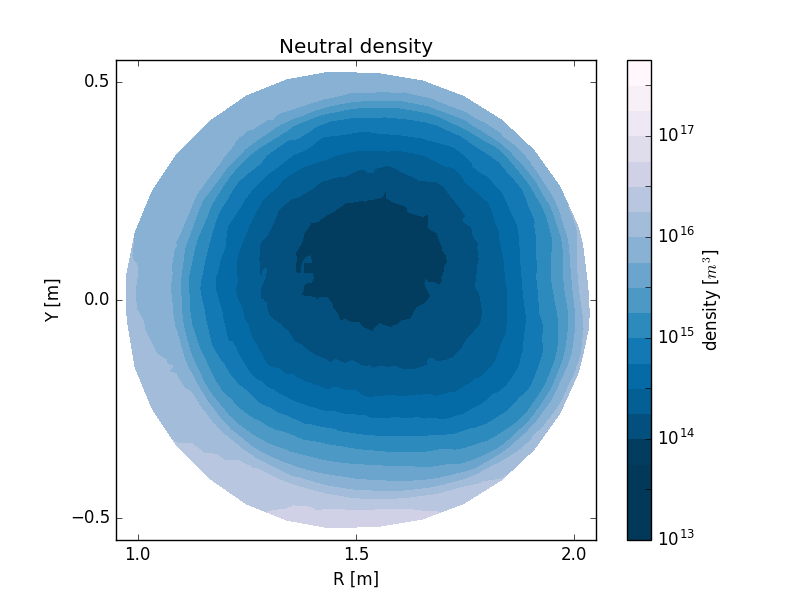
\includegraphics[width = 1.\linewidth]{./plots/degas_neutral_n}
	\label{fig:DEGAS2_2d_density}
	\caption{Typical neutral density result from DEGAS2 show a rapid drop off towards the core. There is two notable asymmetry: the first where the Shafranov shift result in lower neutral density on the outboard side, and the second where the gas puffing that occurs before the PPCD period leaves a residual up/down asymmetry.}
\end{figure}%

DEGAS2, a 2-D Monte Carlo simulation that produces  neutral density and
temperature profiles, was incorporated to model core neutral profiles. DEGAS2
use  $ T_{e} $ and $ n_{e} $ profiles as input, and it tracks and tallies
charge exchange, ionization, recombination, and molecular disassociation
reactions, as well as associated particle and heat flow of test particles.
Synthetic $ D_{\alpha} $ diagnostic are created within DEGAS2, and they are
used to fit experimental measurements of the same, using boundary source rates
as fitting parameters. The precise mechanism behind this neutral source, such
as recycling, is outside of the scope of this work. A three surface source
geometry, each having an independent source rate is used, consisting of an
outboard limiter, a pumping duct region (bottom 45\textdegree) and the rest of
the wall. The outboard limiter is singled out for special attention due to the
Shafranov shift causing the last closed flux surface to strike the outboard
limiter rather than the inboard. The pumping duct being a separate source was
found to be needed to improve the fit quality in PPCD conditions. The sources,
and their contributions to the plasma are assumed to be linearly independent as
neutral-neutral interaction is negligible. An example of the result of the
DEGAS simulation for a single shot and time is shown as fig
\ref{fig:DEGAS2_2D}.

\begin{figure}
	\centering
	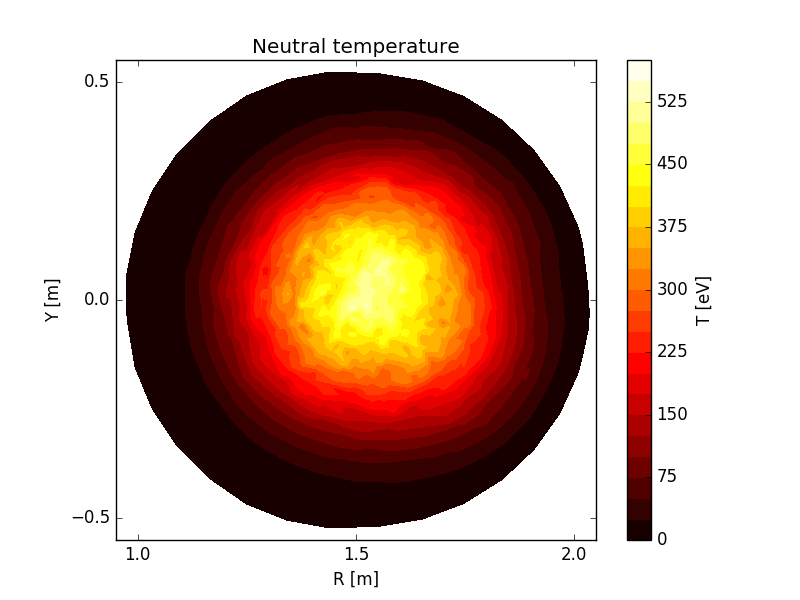
\includegraphics[width = 1.\linewidth]{./plots/degas_neutral_t}
	\label{fig:DEGAS2_2d_temp}
	\caption{Neutral modeling results also show a corresponding 'rise' in temperature as one moves towards the core. This produces a charge exchange loss profile that is both lower and more hollow than previously thought.}
	\label{fig:DEGAS2_2D}
\end{figure}

DEGAS2 simulations are evaluated at 0.5ms intervals despite the forward model
propagates at 1$\mu$s steps.  This timing is chosen due to both the
computational cost of the Monte Carlo simulations, and the frequency at which $
T_e $ measurements, a key input, are available via TS. The 2-D results are
incorporated into the 1-D ion thermal model through flux surface averaging.

DEGAS2 modeling shows $\frac{T_{neutral}}{T_{i}} \simeq 0.7$[[TODO: recheck
this value!!]] in the core, which combined with lower $ n_{neutral} $ leads to
lower charge exchange heat loss than previous estimates. Further, the charge
exchange loss is found have a hollow profile, and is at a level that is broadly
consistent with the temperature evolution of the ions without having to invoke
additional anomalous heating terms during PPCD periods. 

\section{Flow related effects on heat}\label{flow_effects}

In standard MST plasmas, $P_{flow}$ account for $ ~10\% $ of electron heat-loss
\cite{BiewerThesis}, and during PPCD it may become more important as other loss
terms are suppressed. Calculating $P_{flow}$ involves estimating the ion
particle flux.  However, no diagnostic measurements of $n_i$ in MST is
available, therefore, $n_i$ is inferred indirectly through the evolution of
$n_e$ combined with previous work on characterizing the impurity content in
PPCD\cite{Kumar12pop,Nornberg18FST}.

MSTfit uses the 11-chord line integrated $n_e$ measurement from the FIR
interferometer to reconstruct density profile. Measurements show clear rise of
core $n_{e} $in the early half of the PPCD period, ending around 16.5ms. It is
important to determine the nature of this density rise, as the temperature of
these "new" ions would have a significant effect on the model predictions.

The DEGAS2 simulations characterizing the neutral dynamics also provides a
tally of the electron source rate due to the ionization of the neutrals. This
source primarily concentrate in the edge and is too low in the core to account
for the density rise in the core(fig \ref{fig:ne_change}). The further
ionization of impurities due to increasing temperature is another possible
source. Impurity contribution to the electron density rise is estimated using
previous measurements, including carbon, aluminum, oxygen and boron, which were
assumed to be in coronal equilibrium. Their contribution to the electron source
rate is calculated from the change of charge state balance. The result suggests
impurity contribution to $n_e$ rise is insignificant.


\begin{figure}
	\centering
	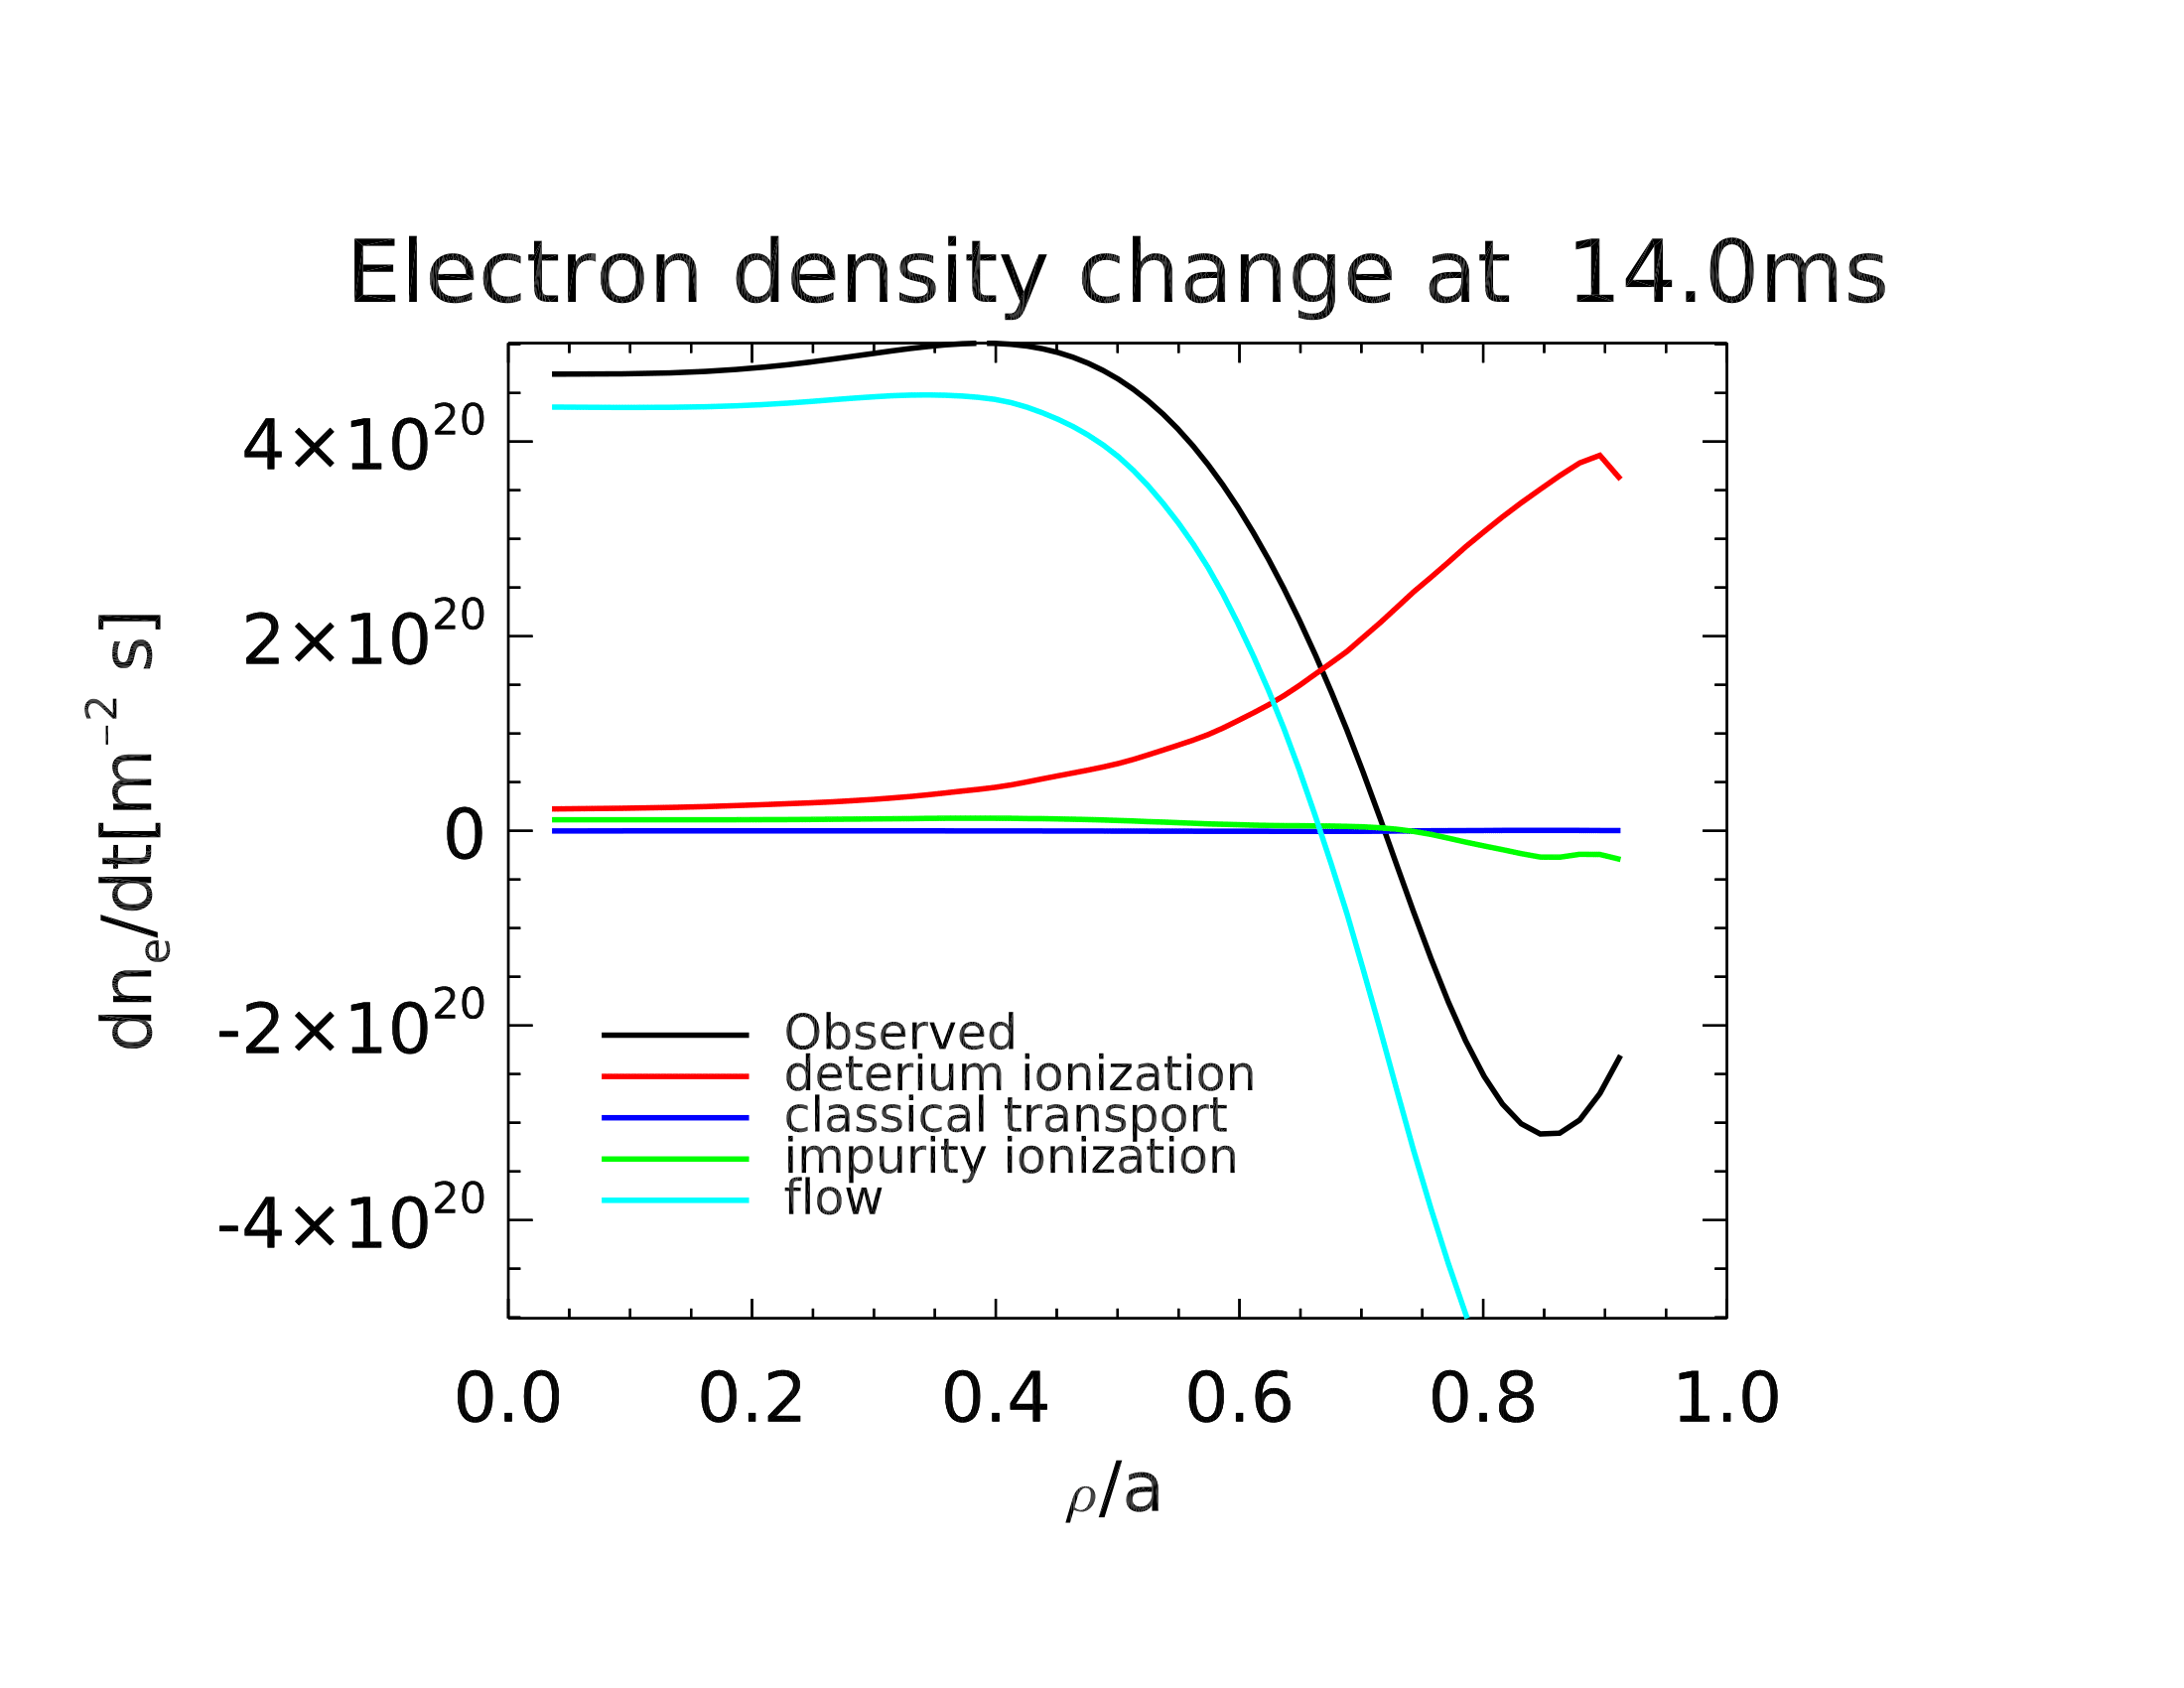
\includegraphics[width=0.95\linewidth]{./plots/dndt_at14-1}	
	\caption{Electron density change show that the $n_e$ source terms are concentrated at the edge, and thus core density rise needs to be accounted for by flux.}
	\label{fig:ne_change}
\end{figure}

\begin{figure}
	\centering
	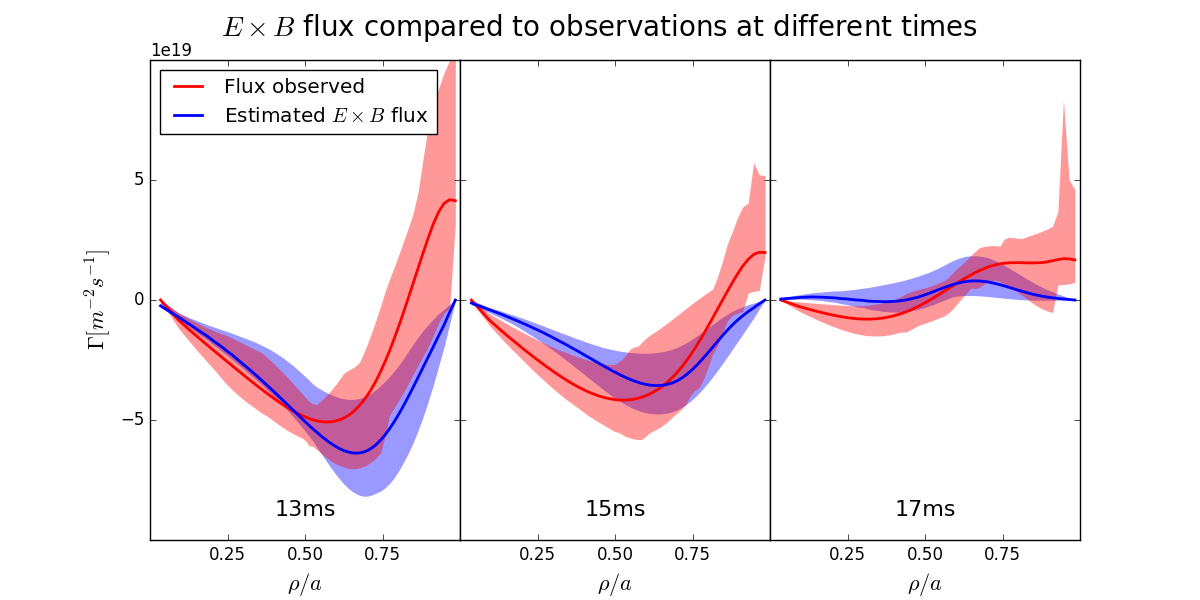
\includegraphics[width=0.95\linewidth]{./plots/flux_comp}
	\caption{Estimated flux values. The calculated $ E\times B $ flux is in red. It goes to zero at the edge as the density goes to zero.}
	\label{fig:flux_compare}


\end{figure}

The calculated electron source rates being insufficient to account for the
density rise, there must be an inward particle flux. The particle flux
($\Gamma_{obs}$) needed to satisfy the continuity equation (\ref{eqn:cont}) is
then calculated. However, we seek to confirm the theoretical plausibility of an
inward pinch by considering the evolution of the magnetic equilibrium.

MST's $\vec{E}$ diagnostic measures plasma potential and does not constrain the
radial $\Gamma_{\vec{E} \times \vec{B}}$. Instead, the slow time-scale E field
is estimated using the evolution of reconstructed B field from edge flux coil
and FIR polarimetry data. The MSTfit equilibrium reconstruction outputs
reconstructed flux values and flux surfaces in 2D which enables 

meaning that $ E_r $ cannot be reconstructed, but as the $ E \times B $ flux of
interest is in the radial direction only $ E_{pol} \text{ and} E_{tor} $ need
to be estimated. In particular $E_{pol}$ can be calculated through:

\begin{align}
E_{pol}(\rho_v) & = \int_{0}^{\rho_v}\rho_v' \frac{dB_{tor}}{dt} d\rho_v'
\end{align}

%where $\rho_v$ is the flux surface averaged minor radius.

$E_{tor}$ is slightly more complicated, as it is in reality a function of major
radius. To incorporate into the 1-D approximation, $E_{tor}(R, Z=0)$ along the
Z = 0 plane is determined as a function of major radius (R) through equation
(\ref{eqn:E_tor}) and boundary condition (\ref{eqn:E_tor_bc}). The results and
then averaged according to flux surface. 

\begin{align}
E_{tor}(R) & = -\frac{1}{\int_{R_0 - a}^{R_0 + a} R' \frac{\partial B_{pol}}{\partial t} dR'} - B_{tor}(R_0 - a) \label{eqn:E_tor}\\
E_{tor} (R_0 - a) & = \frac{- V_{poloidal\ gap} }{2 \pi R}\label{eqn:E_tor_bc}\\
E_{tor}(\rho_v) & = \frac{1}{2}(E_{tor}(R_{in}(\rho_v)) + E_{tor}(R_{out}(\rho_v))
\end{align}
where R refers to the major radius, and r refers to the minor radius from the magnetic axis.

Since the $ \frac{dB}{dt} $ term cannot be evaluated directly, sequential
MSTfit reconstructions, 0.5ms apart is used to provide $ B_{pol} $ and $
B_{tor} $ information from which numerical derivative taken.

$E_{pol}$ is integrated with the boundary condition that the E field is zero at
the magnetic axis. The measured voltage at the inboard poloidal gap provides
the boundary condition of the $ E_{tor} $ integration. The results show it to
be relatively stable in the core, but changes direction in the edge as time
progresses. This reversal correlates with current drive being exhausted in the
edge. Note that the edge $\vec{B}$ field reveres occurs earlier.

From there the radial particle flux is calculated as:

\begin{equation}
\Gamma_{\vec{E} \times \vec{B}} = n_{e} \frac{E_{pol}B_{tor} - E_{tor}B_{pol}}{B^2}
\end{equation}

This is compared to $\Gamma_{implied}$ previously calculated from the
continuity equation in figure \ref{fig:flux_compare}. For the core to about the
mid radius, the estimated $\Gamma_{\vec{E} \times \vec{B}}$ tracks the flux
needed to account for density change well. However, farther in the edge, there
is residual flow outwards since the neutral ionization rates are faster than
density growth, thus particle loss is need to balance the continuity equation.
This is likely cause by anomalous mechanisms such as residual tearing mode or
drift wave activity.

Importantly the $ E_{tor} $ reversal during the PPCD period causes the
estimated $ \Gamma_{\vec{E} \times \vec{B}} $ flow to cease. This echoes MHD
calculations by J. Reynolds that found the $ E \times B $ flow would cease as
the axial E field is reduced and reversed\cite{ReynoldsThesis}.

It is possible to calculate, in lab frame, particle flow's contribution to the
heat balance as well as thermodynamic compression:

\begin{align}
P_{flow} & = -\frac{3}{2}\vec{V}\cdot\vec{\nabla}p - \frac{5}{2}p\cdot\vec{\nabla}\cdot\vec{V}\\
& = -\frac{3}{2}\vec{\nabla}\cdot(nkT\vec{V}) - p\cdot\vec{\nabla}\cdot\vec{V}\label{eq_flux_terms}
\end{align} 

Here pressure $ p = nkT $. In the scope of this work, it is useful to breakout
the thermodynamic work due to compression $  ( p\cdot\vec{\nabla}\cdot\vec{V} )
$ separately from the conservation terms for presentation, like in equation
(\ref{eq_flux_terms}). This is incorporated into the 1-D model by assuming $
\vec{\nabla}\cdot\vec{V}\vert_{\theta, \phi} = 0 \text{ and }
\vec{\nabla}p\vert_{\theta, \phi} = 0 $.


\begin{figure}
	\centering
	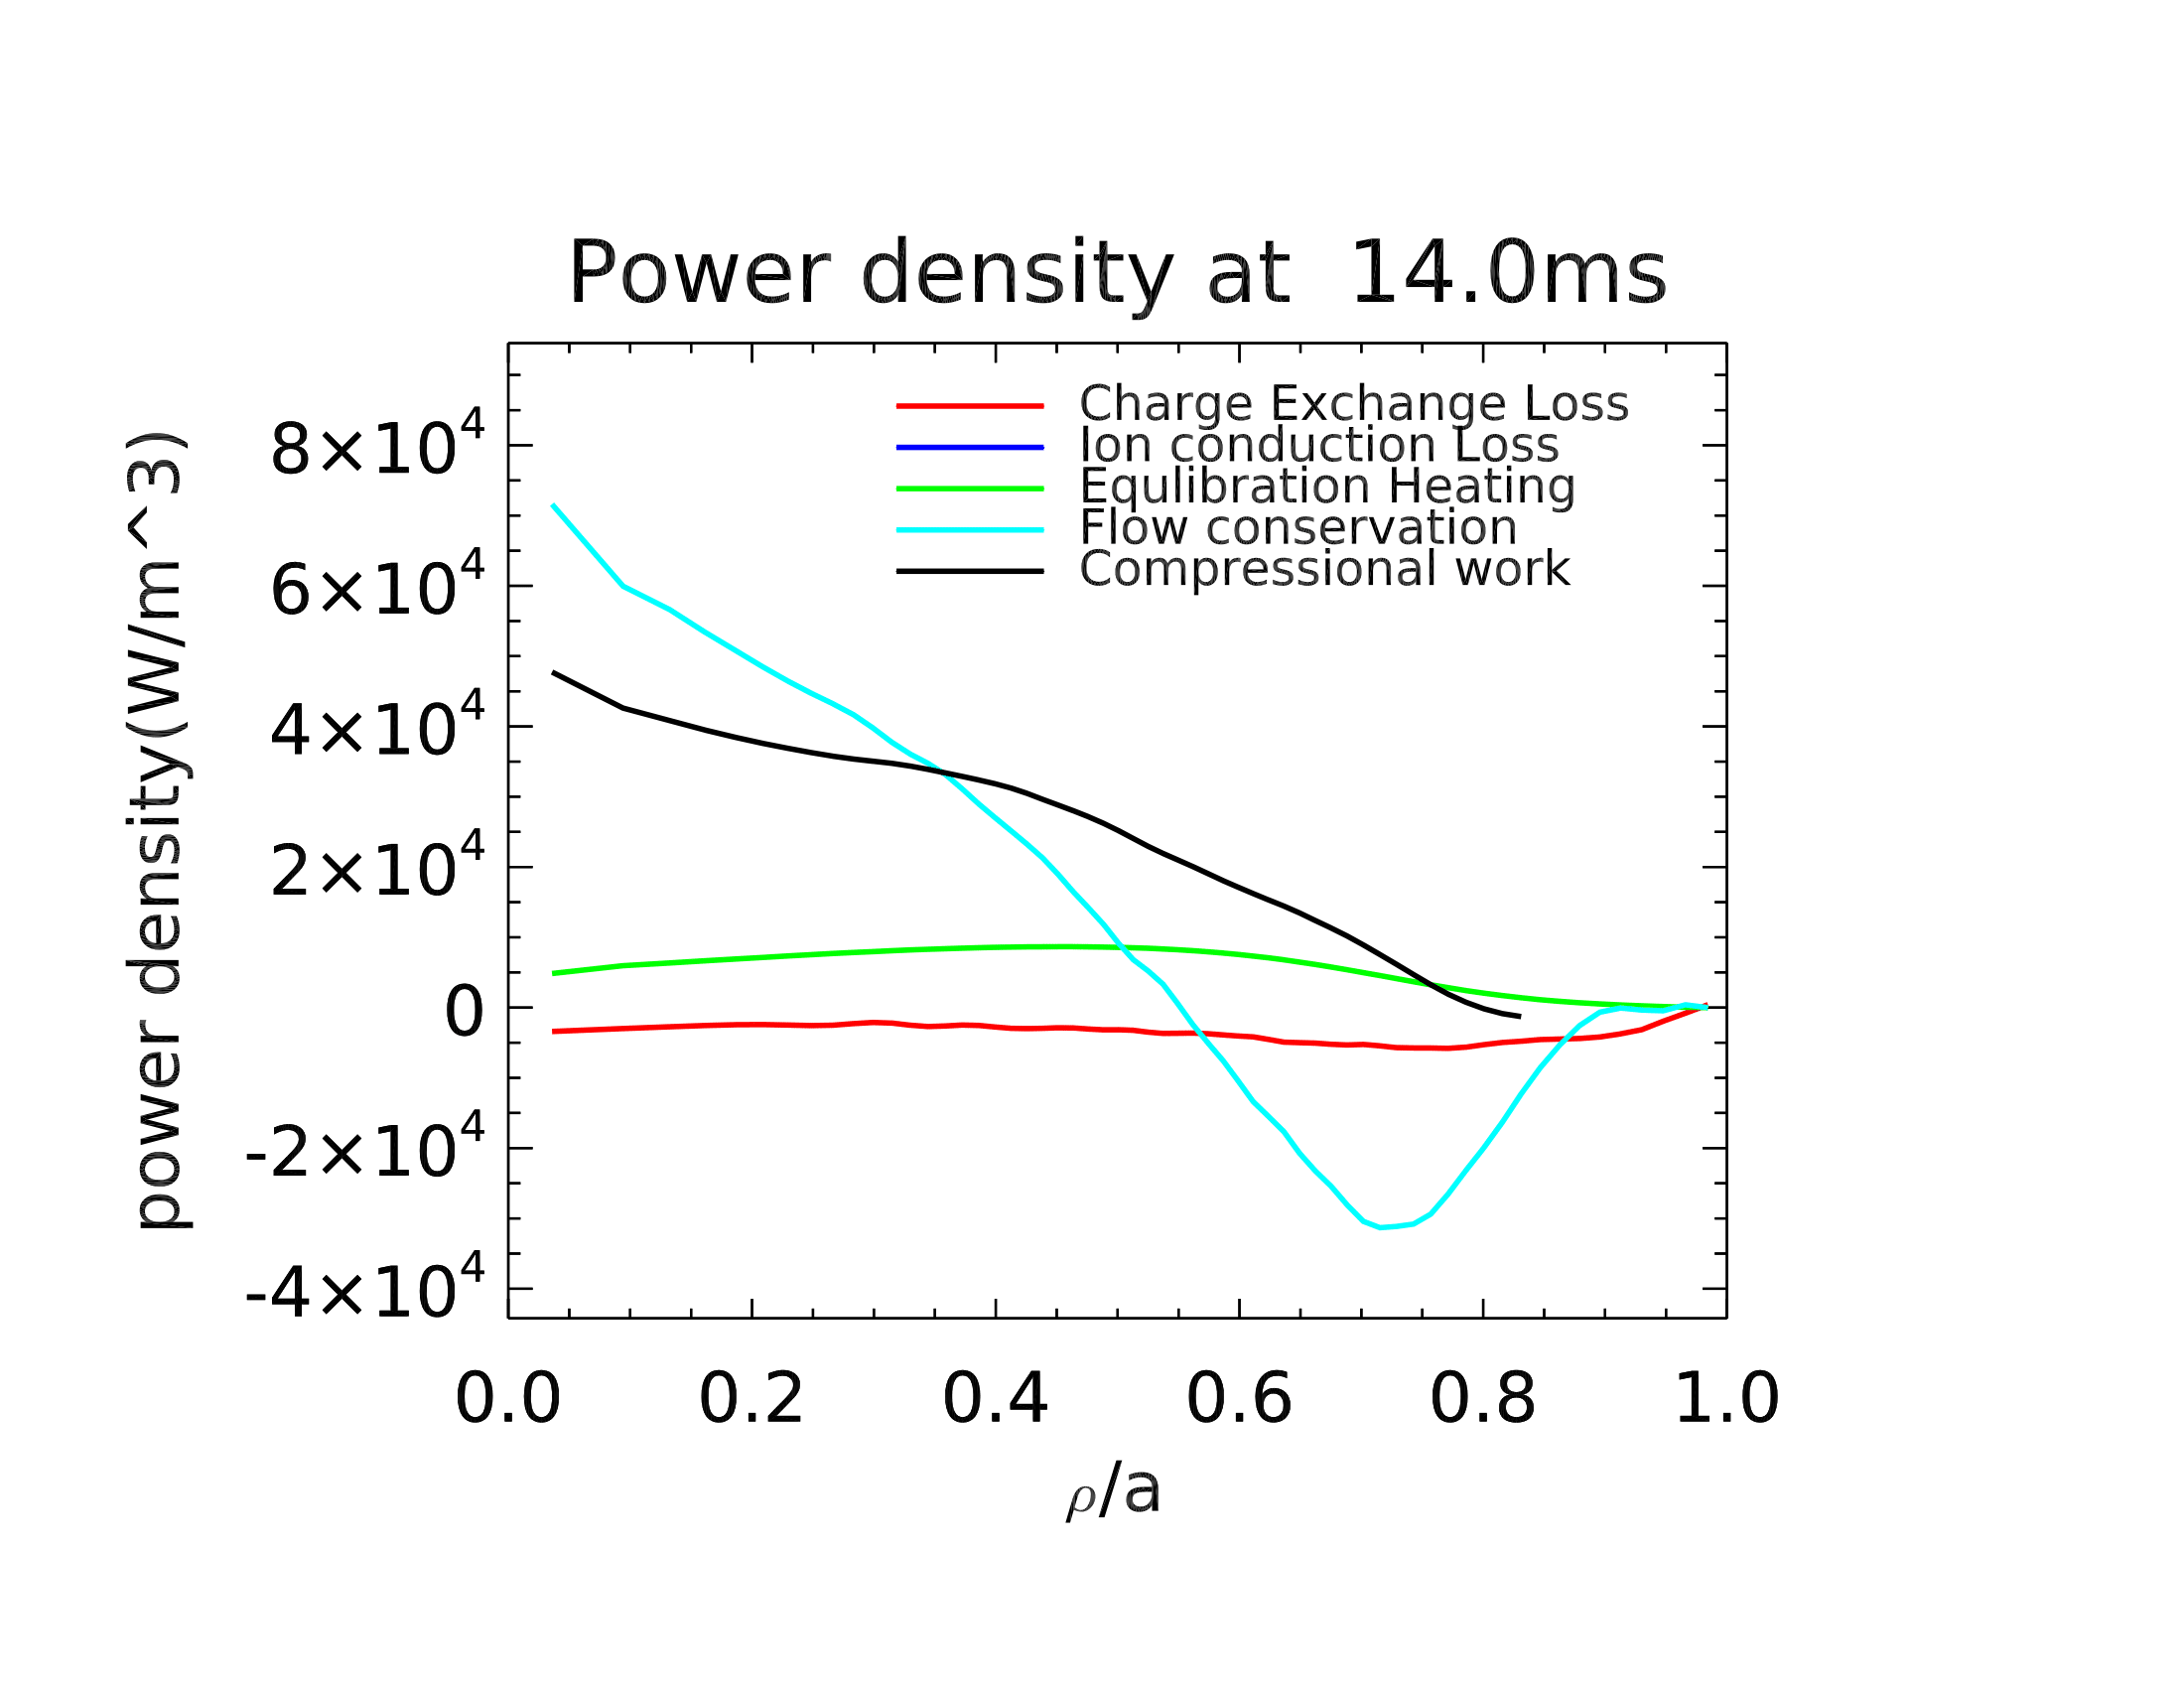
\includegraphics[width=1.\columnwidth]{./plots/dedt_june18-1.png}
	\caption{Flow effects are the most significant.\label{fig:dedt_plot}}
\end{figure}

Using the total implied flux (including $ E \times B $ and anomalous), the flow
contribution to heat balance was calculated and found to be the largest term in
the core of the plasma. Breaking it down further, the notable observation is
that the compression heating is larger than the equlibration heating and is the
largest heating term in the core. The conservation term is larger, but does not
cause temperature rise as it represents the thermal energy being carried by the
pinching particles. The temperature in the core is predicted to rise slightly
while in the gradient region it would decrease as the colder ions flows in.

\section{Results and discussion}

To assess the applicability of the model. It's predictions are compared to
measurements of $T_{C^{6+}}$ using Charge Exchange Recombination
Spectroscopy\cite{DenHartog1994ADynamics,DenHartog1994ADynamics}. CHERS
measurements of C+6 temperature is used as a proxy for majority ion temperature
for model comparisons since $\tau_{C^{+6}-D^{+}}$is small compared to the time
scale of analysis, it is taken as a proxy of majority ion temperature as direct
measurement is not available\cite{Reardon03}, and the primary drive that brings
the two temperatures out of equilibrium are sawtooth events which are
suppressed in PPCD plasmas\cite{Fiksel2009Mass-dependentPlasma}. To begin the
analysis, a ion temperature profile is needed to initialize the model. This is
taken from CHERS measurements at 12ms. Since MST's CHERS system can only
measure temperature at one location at a time, the profile is constructed from
an ensemble of measurements at different locations fitted to a two power
profile across the radius. 12ms being the earliest time that tearing mode is
significantly reduced by PPCD. 

\begin{figure}[!h]
	\centering
	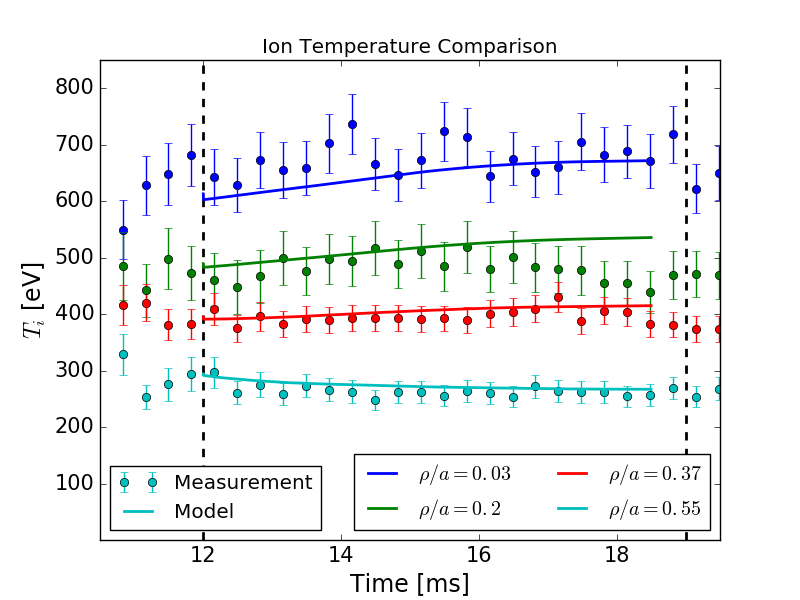
\includegraphics[width=0.95\columnwidth]{./plots/temp_comp_ext}
	\caption{Temperature prediction vs observations. The classical thermal transport model is able to successfully prediction $T_i$ evolution during PPCD up to $\rho /a = 0.55$. Note that model does not initialize at exactly the observed value at a given chord as it is fit to a smooth profile in the radial direction.\label{fig:comp}}
\end{figure}

The model is initialized with $T_i$ profile obtained by fitting CHERS
measurement at 12ms. The time is chosen for being the earliest time that PPCD
consistently suppresses tearing mode activity. The model is then allowed to
propagate until 19ms, and it's prediction of $T_i$ is compared to the
temperature measurement from an ensemble of plasma shots where PPCD was
successful. The result of this comparison is show in fig. \ref{fig:comp}.
Notably the model was able to predict the maintenance and slight rise in
temperature without invoking any anomalous heating. The model, however,
performed poorly in the $\rho /a \approx 0.75$ region.

Previous estimations that resulted in the $T_i$ being considered anomalously
high suffered from the poor estimation of the neutral
interactions\cite{Fiksel2006Confinement}. The calculation used was based on
simple inversions of the $D_{\alpha}$ emission, and it impact the ion transport
calculations in two ways. First, the calculation of the CX loss term, where the
overly high estimate of core $n_n$, as well as the assumption of total loss
(ie. cold neutrals) resulted in overly high estimates of CX loss. Secondly, the
overly high estimates of the source term led to overly high estimates of
outward particle flux, and therefore overly high convective losses. The proper
accounting of the neutral dynamics is therefore crucial to the proper
accounting of thermal transport. Recent development in the Tokamak world also
moving towards more detailed evaluation of the neutrals' impact on transport
calculations by coupling neoclassical PIC code to Monte Carlo neutral transport
code\cite{Stotler2013PedestalCode}.

Neoclassical transport have been ignored in the model since they are expected
to be small for ions in the RFP. Despite the deuterium expected to be in the
banana regime\cite{Kumar12pop} in MST, the neoclassical transport is smaller
than classical as $\frac{q^2}{\epsilon^{3/2}} \leq 0.2$ everywhere in MST.
Another effect that is ignore in this model is the turbulence transport, and
this likely causes the inability for the classical model to predict $T_i$
evolution at $\rho /a \approx 0.75$. Recent studies into turbulence transport
associated with drift wave turbulence in the edge of MST plasma broadly
coincides with this conclusion\cite{NishizawaPRL}.

Further, the successful modeling of tearing suppressed RFP plasma  

We observe strong ion heating associated with magnetic reconnection events in
reversed-field pinch (RFP) plasmas\cite{Gangadhara08}, and it have much faster
characteristic time than ion-electron thermal equlibration. Several mechanisms
have been proposed to account for this anomalous heating including Landau
damping, electron cyclotron damping, stochastic heating, and ion cyclotron
damping\cite{Tangri08}. Further, isolation of the anomalous heating associated
with sawtooth reconnection events, from possible other anomalous heating that
is ongoing during the plasma discharge, is an interesting topic of
investigation. 

This work is supported by the U.S. Department of Energy, Office of Science, and
Office of Fusion Energy Sciences under Award Number DE-FC02-05ER54814.


% If in two-column mode, this environment will change to single-column format so that long equations can be displayed. 
% Use only when necessary.
%\begin{widetext}
%$$\mbox{put long equation here}$$
%\end{widetext}

% Figures should be put into the text as floats. 
% Use the graphics or graphicx packages (distributed with LaTeX2e).
% See the LaTeX Graphics Companion by Michel Goosens, Sebastian Rahtz, and Frank Mittelbach for examples. 
%
% Here is an example of the general form of a figure:
% Fill in the caption in the braces of the \caption{} command. 
% Put the label that you will use with \ref{} command in the braces of the \label{} command.
%
% \begin{figure}
% \includegraphics{}%
% \caption{\label{}}%
% \end{figure}

% Tables may be be put in the text as floats.
% Here is an example of the general form of a table:
% Fill in the caption in the braces of the \caption{} command. Put the label
% that you will use with \ref{} command in the braces of the \label{} command.
% Insert the column specifiers (l, r, c, d, etc.) in the empty braces of the
% \begin{tabular}{} command.
%
% \begin{table}
% \caption{\label{} }
% \begin{tabular}{}
% \end{tabular}
% \end{table}

% If you have acknowledgments, this puts in the proper section head.
%\begin{acknowledgments}
% Put your acknowledgments here.
%\end{acknowledgments}

% Create the reference section using BibTeX:

%\printbibliography
%\bibliography{mst_xing, mendeley_v2}
\bibliography{mst_xing.bib}
\bibliographystyle{apsrev}
\end{document}
%
% ****** End of file aiptemplate.tex ******
